\documentclass[12pt]{article}
\usepackage{geometry}                % See geometry.pdf to learn the layout options. There are lots.
\geometry{letterpaper}                   % ... or a4paper or a5paper or ... 
%\geometry{landscape}                % Activate for for rotated page geometry
\usepackage[parfill]{parskip}    % Activate to begin paragraphs with an empty line rather than an indent
\usepackage{daves,fancyhdr,natbib,graphicx,dcolumn,amsmath,lastpage,url}
\usepackage{amsmath,amssymb,epstopdf,longtable}
\usepackage{paralist}  % need to modify standard enumerate blocks
\DeclareGraphicsRule{.tif}{png}{.png}{`convert #1 `dirname #1`/`basename #1 .tif`.png}
\pagestyle{fancy}
\lhead{CE 3354 -- Engineering Hydrology}
\rhead{SUMMER 2025}
\lfoot{EX1}
\cfoot{}
\rfoot{Page \thepage\ of \pageref{LastPage}}
\renewcommand\headrulewidth{0pt}



\begin{document}
\begin{center}
{\textbf{{ CE 3354 Engineering Hydrology} \\ {Exam 1}}}
\end{center}


\begin{enumerate}

\item For a watershed with a size of $120~km^2$, the following data on precipitation $P$, evaporation
$E$ and runoff $Q$ are recorded in watershed mm.

\begin{table}[h!]
\centering
\caption{Monthly Precipitation (P), Evapotranspiration (E), and Runoff (Q)}
\begin{tabular}{|c|cccccccccccc|}
\hline
\textbf{Month} & Jan & Feb & Mar & Apr & May & Jun & Jul & Aug & Sep & Oct & Nov & Dec \\
\hline
\textbf{P (mm)} & 250 & 205 & 165 & 50 & 5 & 0 & 0 & 5 & 10 & 55 & 65 & 190 \\
\textbf{E (mm)} & 5 & 25 & 30 & 50 & 80 & 100 & 150 & 70 & 60 & 20 & 10 & 5 \\
\textbf{Q (mm)} & 150 & 110 & 80 & 5 & 0 & 0 & 0 & 0 & 0 & 10 & 15 & 120 \\
\hline
\end{tabular}
\end{table}

Determine:
    \begin{enumerate}[a)]
        \item The month (end) when the amount of water stored in the basin is the largest. 
        \item The month (end) when the amount of water stored in the basin is the smallest.
        \item The difference (in $m^3$) in the amount of water stored in the basin between these
two extremes.
        \item The likely climate type (arid, humid temperate or humid tropical) one would expect to find this
catchment.
    \end{enumerate}
\clearpage
%%%%%%%%%%%%%%%%%%%%%%%%%%%%%%%%%%%%%%%%%%%%%%%%%%%%%%%%%%%%
\item A watershed with a catchment area of 1$mi^2$ converts about 60-percent of precipitation into streamflow, the remainder is lost.  The watershed response equation is 

\begin{equation}
 k\frac{dQ}{dt} + Q(t) = P(t) \cdot A \cdot C 
\end{equation}

where $Q(t)$ is the streamflow leaving the catchment, $P(t)$ is the precipitation entering the catchment, $A$ is the catchment area, $C$ is the precipitation to streamflow conversion fraction, and $k$ is the basin characteristic time constant.

\begin{figure}[h!] %  figure placement: here, top, bottom, or page
   \centering
   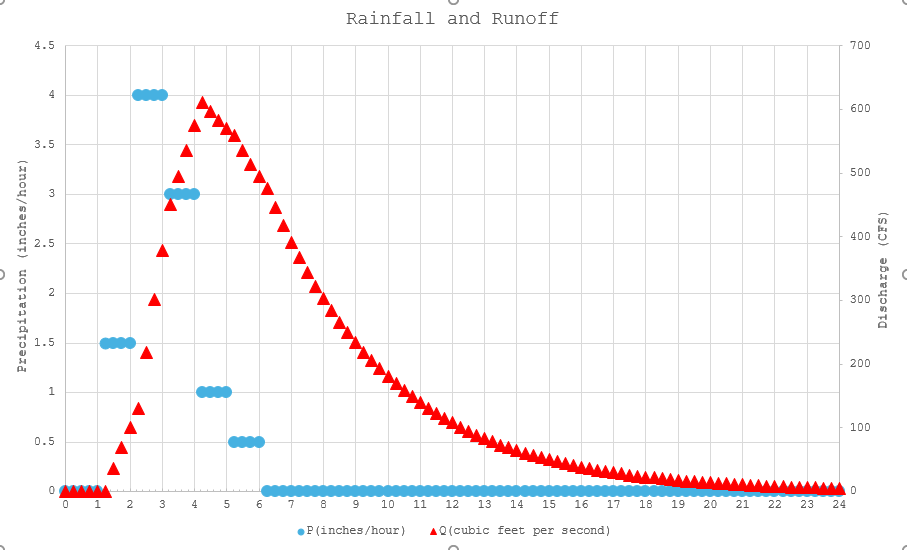
\includegraphics[width=6in]{EX1-P2_PLOT.png} 
   \caption{Rainfall-runoff plot for the catchment}
   \label{fig:EX1-P2-PLOT}
\end{figure}

Using the information in Figure \ref{fig:EX1-P2-PLOT} determine:

    \begin{enumerate}[a)]
        \item The maximum discharge rate in cubic feet per second.
        \item The time when the maximum discharge occurs.
        \item The value in hours of the of the basin time constant $k$.
        \item The total volume in acre feet of precipitation entering the catchment (before any losses)
        \item The total volume in acre feet of discharge leaving the catchment 
    \end{enumerate}

\clearpage
%%%%%%%%%%%%%%%%%%%%%%%%%%%%%%%%%%%%%%%%%%%%%%%%%%%%%%%%%%%%
\item design storm

\clearpage
%%%%%%%%%%%%%%%%%%%%%%%%%%%%%%%%%%%%%%%%%%%%%%%%%%%%%%%%%%%%
\item The relation between infiltration capacity in mm/hour and the time (in hours) since the
start of the experiment as measured with an infiltrometer is depicted in Figure \ref{fig:INFIL}. 

\begin{figure}[h!] %  figure placement: here, top, bottom, or page
   \centering
   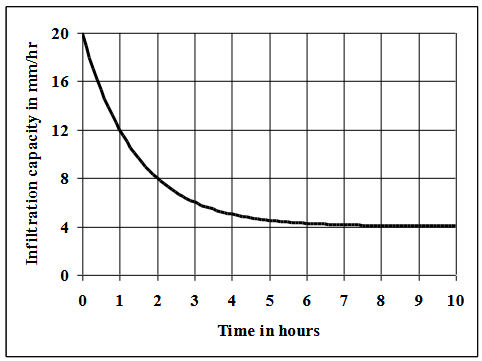
\includegraphics[width=5in]{INFIL.png} 
   \caption{Infiltrometer data for some soil}
   \label{fig:INFIL}
\end{figure}

The relationship is to be described with the Horton infiltration model 
\begin{equation}
q(t)=f_c+(f_o-f_c)e^{-kt}
\end{equation}

Determine:
    \begin{enumerate}[a)]
        \item The equilibrium infiltration rate, $f_c$, in mm/hr.
        \item The initial (dry soil) infiltration rate, $f_o$, in mm/hr.
        \item The soil constant $k$.
        \item The total amount of water that will infiltrate into an initially dry soil during a rainstorm with a duration 60 minutes and a constant intensity of 20 mm/h.
        \item The total amount of water that will infiltrate into an initially dry soil during a rainstorm with a duration 480 minutes and a constant intensity of 12 mm/h.
    \end{enumerate}

\end{enumerate}



\end{document}  